\chapter{Results}

We performed our test runs on a standalone cluster, consisting of 4 nodes, with 32 cores each. We configured the Apache Flink framework until we found the configuration that provided the best performance. Once we hit our limitation of hard disk size, we created an alternative method to measure the time of feature extraction. This allows to have an idea of the actual time the feature extraction requires without the increased delay of writing to a hard disk.


\section{CSV File Method}

Figure 4.1 one shows the average execution time as the input increases, while keeping the cores at 128.

\begin{figure}[ht]
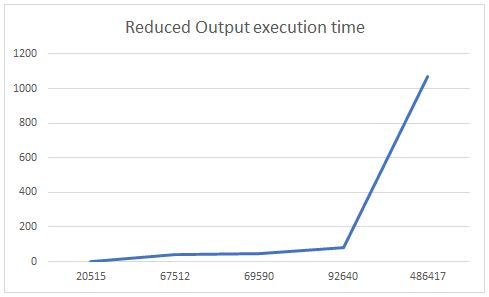
\includegraphics[width=12cm]{Thesis/figures/figure3.JPG}
\caption{On X-Axis we see the number of Unique\newline Nodes. On Y-Axis we see the average time in minutes. }
\label{fig:graph}
\end{figure}


The other objective we had was regarding strong scaling. We measured the speedup we can achieve given a fixed size input, by increasing our resources. Figure 4.2 shows the execution times on a specific data set, when we increase the cores from 32 to 128.

\begin{figure}[ht]
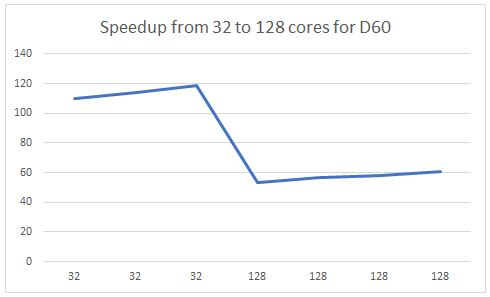
\includegraphics[width=12cm]{Thesis/figures/figure2.JPG}
\caption{Execution Time from 32 to 128 cores.}
\label{fig:graph}
\end{figure}


\newpage
\section{Reduced Output Method}
Our test results on reduced output method, showed that writing the complete csv file took (and still takes even though the size is smaller) a significant amount. What we observe at Figure 4.3 that if Flink implements a way to train the LR model or we use a method to redirect the features using data pipelines, will have a really good performance and great scalability. 

\begin{figure}[ht]
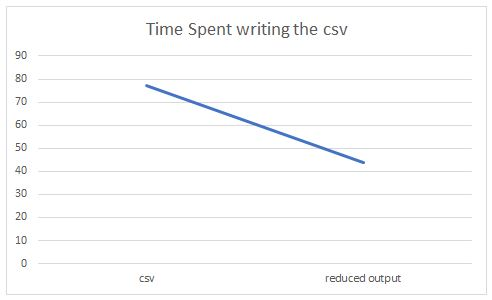
\includegraphics[width=10cm]{Thesis/figures/figure4.JPG}
\caption{time saved just by reducing the output file by a factor of 100.}
\label{fig:graph}
\end{figure}

Finally we show at figure 4.4 that we were able to increase the unique ids used earlier by almost 700\% until we hit our limitations with hard disk space. 

\begin{figure}[ht]
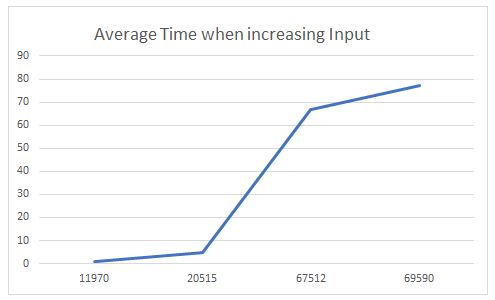
\includegraphics[width=10cm]{Thesis/figures/figure5.JPG}
\caption{Input data scaling.}
\label{fig:graph}
\end{figure}



% Replace with your text
%https://www.tablesgenerator.com/?fbclid=IwAR0W039IFX2-HUWOTwVTY_-CraF2DvdBtIlM6pCGMOZHgLBfQkyjM_V5TZY